%----------------------------------------------------------
% report_temp.tex
% v1.0
% 2022/10/28
% by Carlos Rodríguez - Pardo, 2023, Universidad Carlos III de Madrid
% ----------------------------------------------------------

\documentclass{wsdcr}
\usepackage[spanish]{babel}


\title{Análisis Avanzado de Datos - Práctica Final}
\author{Dario, Muñoz Muñoz (NIA: 100405982)}
\date{\today}

\begin{document}

\maketitle

\section{Introducción}
Spotify es una plataforma de streaming de música que ofrece a sus usuarios acceso a millones de canciones de diversos géneros y épocas. Para mejorar la experiencia de los usuarios, Spotify utiliza la inteligencia artificial (IA) para analizar las características acústicas y la popularidad de las canciones, y así poder ofrecer recomendaciones personalizadas, listas de reproducción y radios. El conjunto de datos Spotify Dataset 1921-2020, 600k+ Tracks recoge información sobre más de 600 mil canciones publicadas entre 1921 y 2020, incluyendo datos como el nombre, los artistas, la fecha de lanzamiento, la duración, la presencia de contenido explícito y varios atributos acústicos como la bailabilidad, la energía o el tempo. En este trabajo se pretende explorar este conjunto de datos utilizando dos tipos de aprendizaje automático: el supervisado y el no supervisado. El primero se basa en utilizar datos etiquetados para entrenar un modelo que pueda predecir la salida o la clase de nuevos datos. El segundo se basa en utilizar datos sin etiquetar para descubrir patrones ocultos o agrupaciones en los datos. El objetivo es aplicar ambos tipos de aprendizaje para obtener información relevante sobre las canciones y sus características.

Para el aprendizaje supervisado, nos centraremos en predecir la popularidad de las canciones a partir de sus atributos acústicos. La popularidad es un valor numérico entre 0 y 100 que indica el grado de éxito o reconocimiento de una canción en Spotify.

Para el aprendizaje no supervisado, nos centraremos en agrupar las canciones por su danzabilidad a partir de sus atributos acústicos. La danzabilidad es una categoría que describe el grado de facilidad para bailar la canción.

\section{Dataset}

El dataset escogido es de Yamac Eern AY y se llama "Spotify Dataset 1921-2020, 600k+ Tracks". Contiene 600 mil canciones lanzadas entre 1921 y 2020. Este dataset puede ser usado para tareas de aprendizaje supervisado y no supervisado, como clasificación, regresión o agrupamiento. El dataset contiene dos archivos, uno llamado "tracks.csv" tiene 20 columnas con los siguientes datos:

\begin{itemize}
    \item \textbf{id}: el identificador único de cada canción en Spotify (cadena alfanumérica).
    \item \textbf{name}: el nombre de la canción (cadena de texto).
    \item \textbf{popularity}: el nivel de popularidad de la canción en una escala de 0 a 100 (número entero).
    \item \textbf{duration\_ms}: la duración de la canción en milisegundos (número entero).
    \item \textbf{explicit}: si la canción tiene contenido explícito o no (0 = no, 1 = sí) (número binario).
    \item \textbf{artists}: los artistas que participan en la canción (lista de cadenas de texto).
    \item \textbf{id\_artists}: los identificadores únicos de los artistas en Spotify (lista de cadenas alfanuméricas).
    \item \textbf{release\_date}: la fecha de lanzamiento de la canción en formato YYYY-MM-DD (cadena de texto).
    \item \textbf{danceability}: el grado de facilidad para bailar la canción en una escala de 0 a 1 (número decimal).
    \item \textbf{energy}: el nivel de energía e intensidad sonora de la canción en una escala de 0 a 1 (número decimal).
    \item \textbf{key}: la tonalidad musical principal de la canción en una escala cromática estándar que va del 0 al 11, donde el 0 es Do y el 11 es Si (número entero).
    \item \textbf{loudness}: el nivel promedio del volumen sonoro en decibeles (dB) durante toda la canción (número decimal negativo o cero).
    \item \textbf{mode}: el modo musical principal de la canción, donde el 0 es menor y el 1 es mayor (número binario).
    \item \textbf{speechiness}: el grado en que se habla o se canta durante la canción en una escala del 0 al 1, donde valores cercanos al cero indican más música instrumental y valores cercanos al uno indican más voz humana (número decimal).
    \item \textbf{acousticness}: el grado en que se usan instrumentos acústicos o eléctricos durante la canción en una escala del 0 al uno, donde valores cercanos al cero indican más instrumentos eléctricos y valores cercanos al uno indican más instrumentos acústicos (número decimal).
    \item \textbf{instrumentalness}: el grado en que se usan instrumentos musicales o voces humanas durante la canción en una escala del cero al uno, donde valores cercanos al cero indican más voces humanas y valores cercanos al uno indican más instrumentos musicales(número decimal).
    \item \textbf{liveness}: el grado en que se percibe que hay público presente durante la grabación o reproducción de la canción en una escala del cero al uno, donde valores cercanos al cero indican menos presencia pública y valores cercanos al uno indican más presencia pública(número decimal).
    \item \textbf{valence}: el grado en que se transmite un sentimiento positivo o negativo durante la canción en una escala del cero al uno, donde valores cercanos al cero indican sentimientos más negativos como tristeza o ira y valores cercanos al uno indican sentimientos más positivos como alegría o euforia(número decimal).
    \item \textbf{tempo}: el ritmo promedio expresado como las pulsaciones por minuto(BPM) durante toda la canción(número decimal).
    \item \textbf{time\_signature}:el número promedio expresado como fracciones simples(4/4 ,3/4 , etc.)de las pulsaciones por compás musical durante toda la canción(número entero).
\end{itemize}

Este dataset es muy útil para analizar las tendencias musicales a lo largo del tiempo y las preferencias del público. También puede servir para generar recomendaciones personalizadas o crear nuevas composiciones musicales basadas en los atributos acústicos.

\section{Análisis del Dataset}

Para realizar un buen análisis de datos del Dataset, primero mostraremos la matriz de correlación y la explicaremos. La matriz de correlación nos permite ver la relación lineal entre las variables numéricas del Dataset. Algunas de las correlaciones más destacadas son:

\begin{itemize}
    \item La variable loudness tiene una alta correlación positiva con la variable energy (0.76), lo que indica que a mayor intensidad sonora, mayor nivel de energía percibida en las canciones.
    \item La variable valence tiene una moderada correlación positiva con la variable danceability (0.53), lo que sugiere que a mayor grado de positividad o alegría expresada en las canciones, mayor facilidad para bailarlas.
    \item La variable acousticness tiene una alta correlación negativa con la variable energy (-0.72) y una moderada correlación negativa con la variable loudness (-0.52), lo que implica que a mayor presencia de elementos acústicos en las canciones, menor nivel de energía y menor intensidad sonora.
\end{itemize}

Estos resultados nos permiten conocer mejor las características y relaciones entre las variables del Dataset y nos ayudan a entender mejor las características de las canciones del Dataset y a identificar posibles patrones o tendencias.

\begin{figure}[h!] 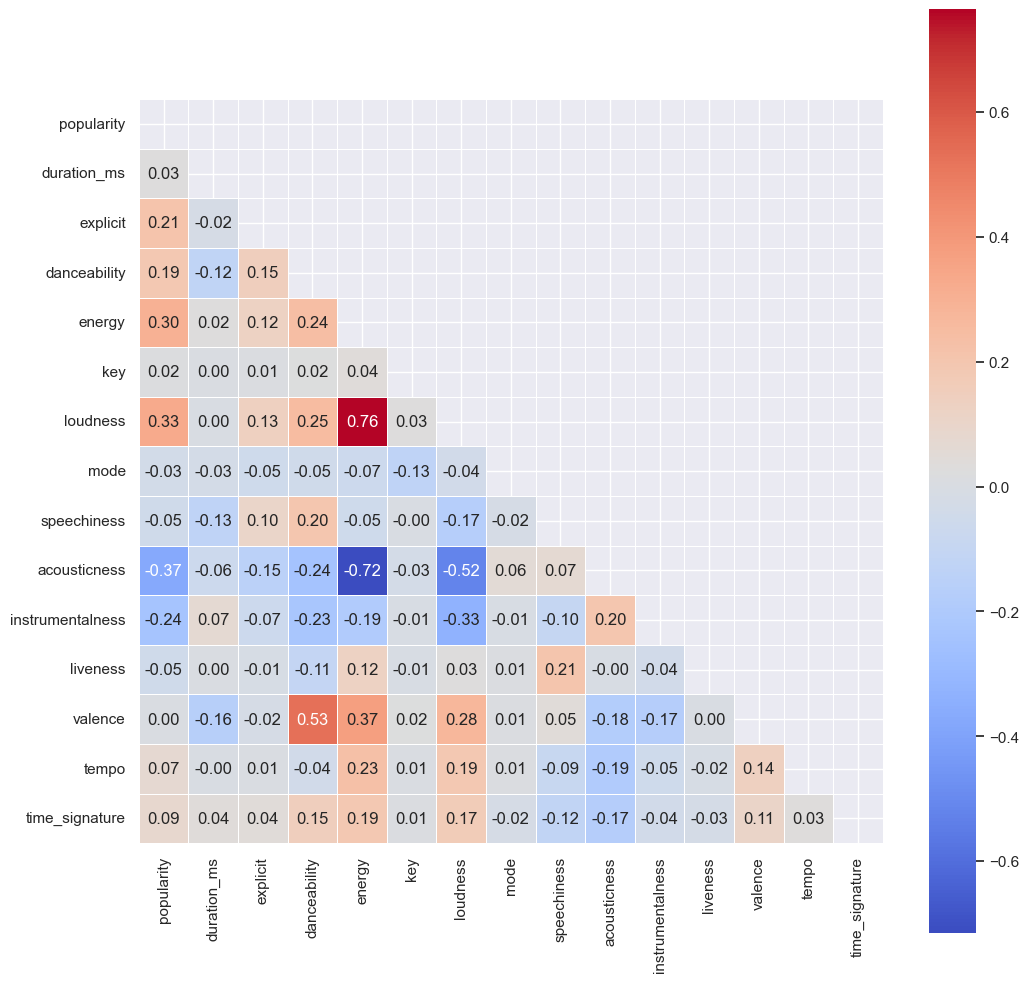
\includegraphics[width=\columnwidth]{images/matriz_correlacion.png} \caption{Matriz de correlación} \label{fig:matriz_correlaccion} \end{figure}

También para analizar el dataset realizaremos un histograma en la \figurename{\ref*{fig:histogramas}}, de cada variable que vamos a predecir, es decir popularidad y danzabilidad. Esto para ver cómo están distribuidas estas variables en el dataset.


\begin{figure}[h!] 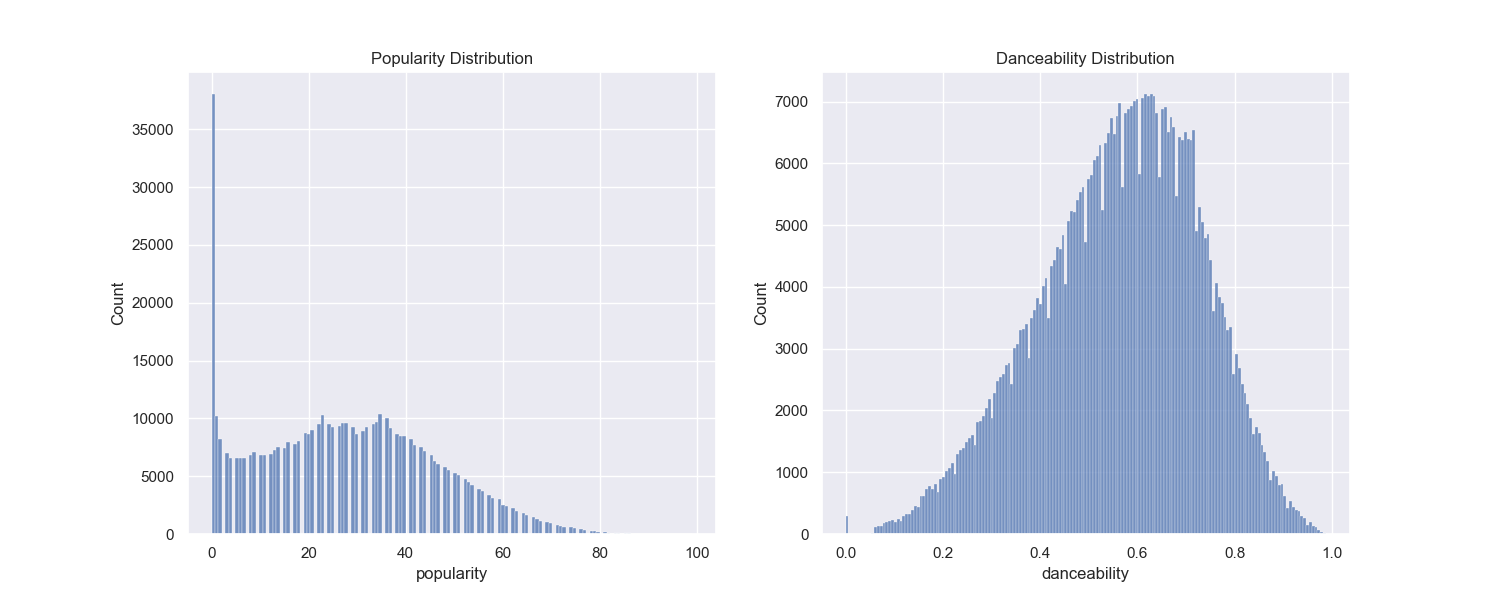
\includegraphics[width=\columnwidth]{images/histogramas.png} \caption{Histograma de popularidad y danzabilidad} \label{fig:histogramas} \end{figure}


También se ha realizado una comparación entre variables representativas como son la popularidad y la intensidad sonora, en la \figurename{\ref*{fig:relacion popularidad e intensidad sonora}}. en este se puede ver que tienen más popularidad las canciones con mayot intensidad sonora.

\begin{figure}[h!] 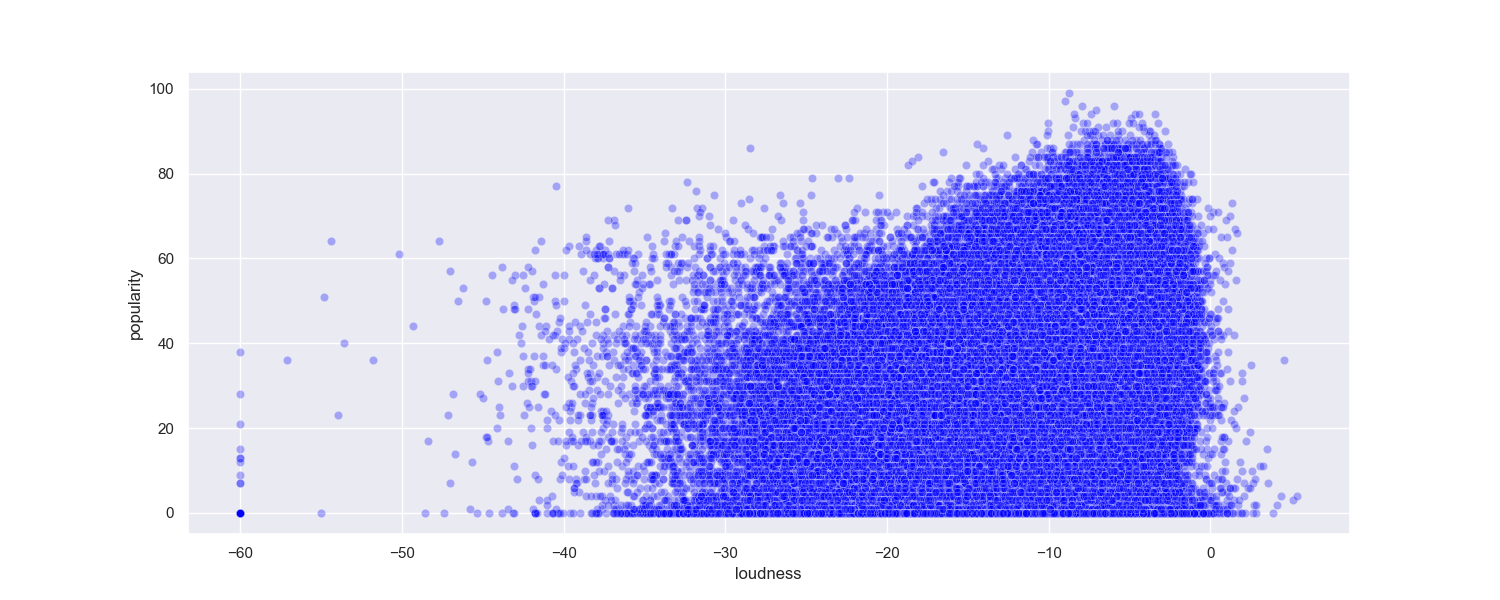
\includegraphics[width=\columnwidth]{images/popularity_loudness_scatterplot.png} \caption{Relación de popularidad e intensidad sonora} \label{fig:relacion popularidad e intensidad sonora} \end{figure}

Por último también se ha realizado una comparación entre las variables bailabilidad y cuanto se habla en una canción en la \figurename{\ref*{fig:relacion danzabilidad y locuencia}}. Viéndose que la mayoría de las canciones con mayor nivel de danzabilidad tienen muy poca locuencia.

\begin{figure}[h!] 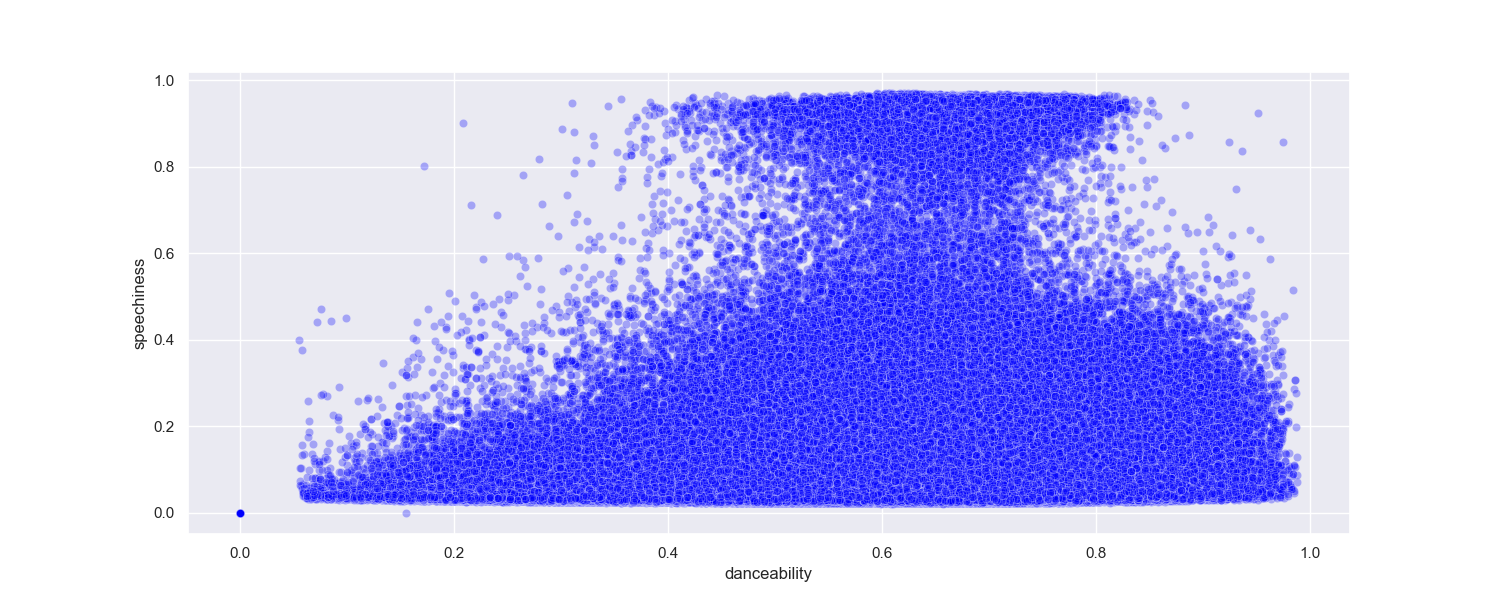
\includegraphics[width=\columnwidth]{images/danceability_speechiness_scatterplot.png} \caption{Relación de danzabilidad y locuencia} \label{fig:relacion danzabilidad y locuencia} \end{figure}

\section{Método}
Primero se realizará un preprocesado de los datos eliminando algunos inservibles, y quedándonos solo con: energy, liveness, tempo, valence, loudness, speechiness, acousticness, danceability, instrumentalness. A continuación se realizara una normalización de los datos que no se encuentran entre 0 y 1 que serian popularity, loudness y tempo.
\subsection{Aprendizaje supervisado}
Para el aprendizaje supervisado primero se dividirá el dataset en dos grupos train y test con una division de 70 a 30. Este aprendizaje se realizará mediante técnicas de regresión. Las elegidas han sido: Simple Linear Regression, KNeighborsRegressor, RandomForestRegressor y una red neuronal de TensorFlow. Una vez entrenado el modelo, este se evaluará con el conjunto de test para obtener diferentes métricas que sirvan como comprobación de que el modelo está funcionando correctamente.
Como mas adelante se explicara, en la sección de resultados, los conseguidos no son lo suficientemente satisfactorios, por lo que se tomara otro enfoque a este problema. En vez de usar regresión, se calificara entre popular y no popular a las canciones, haciendo esta etiquetación a partir de el valor 0.41 de popularidad que se encuentra en el 75\% de los datos. Y seguido de esto se realizara un balanceo de las clases ya que al dividirlo en 75\% y 25\%se han desbalanceado las clases.
\subsection{Aprendizaje no supervisado}
TODO
Respecto al aprendizaje no supervisado se aplicaran técnicas de clustering y de reducción de dimensionalidad. El clustering nos ayudará a ver cómo está segmentado el mercado y en que se fijan los consumidores y con la reducción de dimensionalidad conseguiremos hacer un modelo más pequeño sin tantas variables pero con una eficacia muy parecida.

\section{Resultados}
\subsection{Aprendizaje supervisado}
\begin{table}[t]
    \begin{center}
        \begin{tabular}{| c | c | c | c | }\hline
            Modelo                   & $R^{2}$ & MSE    & MAE    \\ \hline
            Simple Linear Regression & 0.2089  & 0.0264 & 0.1319 \\
            KNeighborsRegressor      & 0.2065  & 0.0290 & 0.1357 \\
            RandomForestRegressor    & 0.3482  & 0.0230 & 0.1199 \\
            Red neuronal TensorFlow  & 0.2986  & 0.0244 & 0.1253 \\ \hline
        \end{tabular}
        \caption{Resultados supervisado regresión}
        \label{tab:resultados supervisado regresion}
    \end{center}
\end{table}


\begin{table}[t]
    \begin{center}
        \begin{tabular}{| c | c | c | c | }\hline
            Modelo                  & Accuracy & Precision & F1 score \\ \hline
            KNeighborsClassifier    & 0.6000   & 0.5968    & 0.5944   \\
            RandomForestClassifier  & 0.6894   & 0.6932    & 0.6803   \\
            AdaBoostClassifier      & 0.6791   & 0.6827    & 0.6587   \\
            DecisionTreeClassifier  & 0.6702   & 0.6890    & 0.6112   \\
            GaussianNB              & 0.6449   & 0.7138    & 0.4732   \\
            MLPClassifier           & 0.6761   & 0.7021    & 0.6008   \\
            Red neuronal TensorFlow & 0.6758   & 0.7021    & 0.6475   \\ \hline
        \end{tabular}
        \caption{Resultados supervisado clasificación}
        \label{tab:resultados supervisado clasificacion}
    \end{center}
\end{table}

\subsection{Limitaciones}

\section{Conclusiones y Trabajo Futuro}

\appendices
\section{}
Appendix uno va aquí.

% you can choose not to have a title for an appendix
% if you want by leaving the argument blank
\section{}
Appendix dos va aquí.


% use section* for acknowledgment
\bibliographystyle{IEEEtran}
%% you can change the style into any other styles available, I personally love IEEEtran.
\bibliography{citations}
%% to generate references, input the name of your .bib file and cite anywhere in the document.


\end{document}
